\documentclass[10pt,a4paper]{article}
\usepackage[utf8]{inputenc}
\usepackage[T1]{fontenc}
\usepackage{amsmath}
\usepackage{amsfonts}
\usepackage{amssymb}
\usepackage{graphicx}
\usepackage{epstopdf}

\usepackage{listings}
\usepackage{color}
\usepackage{tikz}
\usetikzlibrary{arrows}
\usepackage{hyperref}

\title{DD2200 - Operativsystem \\ Laboration 3 \\ Minneshantering v.4 \\ Period 4, läsår 2014}
\author{Carl Svensson, F-10 \\ 910414-1412 \\ carlsven@kth.se}
\date{}

\definecolor{dkgreen}{rgb}{0,0.6,0}
\definecolor{gray}{rgb}{0.5,0.5,0.5}
\definecolor{mauve}{rgb}{0.58,0,0.82}

\lstdefinestyle{cstyle}{%
  language=C,
  aboveskip=3mm,
  belowskip=3mm,
  showstringspaces=false,
  columns=flexible,
  basicstyle={\small\ttfamily},
  numbers=none,
  numberstyle=\color{mauve},
  keywordstyle=\color{blue},
  commentstyle=\color{dkgreen},
  stringstyle=\color{mauve},
  breaklines=true,
  breakatwhitespace=true
  tabsize=3
}

\lstdefinestyle{bashstyle}{%
  language=C,
  aboveskip=3mm,
  belowskip=3mm,
  showstringspaces=false,
  columns=flexible,
  basicstyle={\small\ttfamily},
  numbers=none,
  numberstyle=\color{mauve},
  keywordstyle=\color{blue},
  commentstyle=\color{dkgreen},
  stringstyle=\color{mauve},
  breaklines=true,
  breakatwhitespace=true
  tabsize=3
}

\lstset{
  style=bashstyle
}

\begin{document}

\maketitle
\tableofcontents
\clearpage

\section{Problembeskrivning}

Uppgiften består av att implementera en minneshanterar i form av funktionerna malloc(), free() och realloc(). Funktionerna ska välja samma gränssnitt de vanliga motsvarande funktionerna. Implementationen ska sedan testas så att den är korrekt och prestandan ska utvärderas.

\subsection{Förberedelsefrågor}

Koden innanför "\#ifdef MMAP" deklarerar en variabel "\_\_endHeap" som håller koll på var slutet på heapen är samt funktionalitet för att initialisera den variabeln. Variabeln används sedan för att allokera mer minne som försöker placeras så nära slutet av heapen som möjligt för att minska fragmentering.

\begin{enumerate}
\item Utan initialisering kommer \_\_endHeap peka på adress 0 vilket är nära heapens bas.
\item Kerneln väljer helt själv var minnet placeras. Funktionen kommer returnera adressen till där minnet faktiskt placeras.
\item Väljer man inte MAP\_SHARED så blir det istället MAP\_PRIVATE vilket betyder att det är en "copy-on-write"-mappning av minnet vilket betyder att ändringar inte är synliga för andra processer som mappar till samma minne.
\end{enumerate}

\section{Programbeskrivning}

Implementationen håller en länkad lista med lediga block. Varje block består av en eller flera sidor som har allokerats med mmap(). I början av ett block finns en 64 byte stor header. Headern innehåller en pekare till nästa block, blockets storlek samt ett kontrollvärde som gör att det går att kontrollera att blocket verkligen har allokerats med malloc(). Att headern är just $64=2^6$ byte gör att aritmetik med sidstorlekar blir lättare då headerns storlek delar sidstorleken.

Implementationen kan köras med två olika strategier, first-fit och best-fit. Listan börjar med att dummy-block av storlek 0 som allokeras på stacken. Vid anrop till malloc() så gås listan igenom i jakt på en kandidat. Om en kandidat hittas och är exakt rätt storlek så väljs den, oavsett strategi. Om blocket är större så används det ändå vid first-fit. Vid best-fit så sparas den som potentiell kandidat om den passar bättre än den tidigare kandidaten.

När listan gåtts igenom ett varv så tas används den nuvarande kandidaten vid best-fit. Om vi kör first-fit eller inte har hittat någon kandidat så betyder det att mer minne måste allokeras. Då anropas mmap() och ett nytt block initieras. Samtidigt flyttas heapens slut framåt. Detta block stoppas in i ledighetslistan med hjälp av free() innan malloc() sen kan fortsätta leta och då direkt hitta det.

När free() anropas kontrolleras först att blocket är giltigt genom att kontrollera att pekaren ligger i heapen och att kontrollvärdet finns i headern. Om allt är ok så stoppas blocket in i listan på rätt plats. Om blocket angränsar till block så slås dessa ihop för att motverka fragmentering.

När realloc() anropas körs först malloc() följt av memcpy() och free(). Under denna process gärs även lite kontroller som att kontrollera att malloc() lyckas och att det som ska reallokeras är giltigt minne.

\clearpage
\subsection{Testkörning}

För att testa korrektheten testades implementationen med de givna testerna som kördes ett flertal gånger och klarade samtliga tester, inklusive de "avancerade".

För att sedan mäta prestandan så kördes mina två implementationer samt systemets med testprogrammet som hittas i källkodsavsnittet. Programmet allokerar, frigör och omallokerar slumpmässigt stora block av minne. Varje körning gjordes 10 gånger där programmet kördes med 1, 10, 100, 1000, 10000 resp. 100000 iterationer. Detta upprepades även med 0\%, 10\%, 20\%, 30\%, 40\% samt 50\% reallokeringsanrop. Resultaten visas i graferna nedan på logaritmerade skalor.

Som man kan se så påverkade inte andelen realloc resultatet märkbart. Detta är inte så förvånande då det bara är två anrop till malloc() respektive free() med lite extra kontroller.

Vi ser även i jämförelsen att first-fit och best-fit presterade ungefär lika bra men att de båda presterade något sämre än systemets implementation.

\clearpage

\begin{figure}
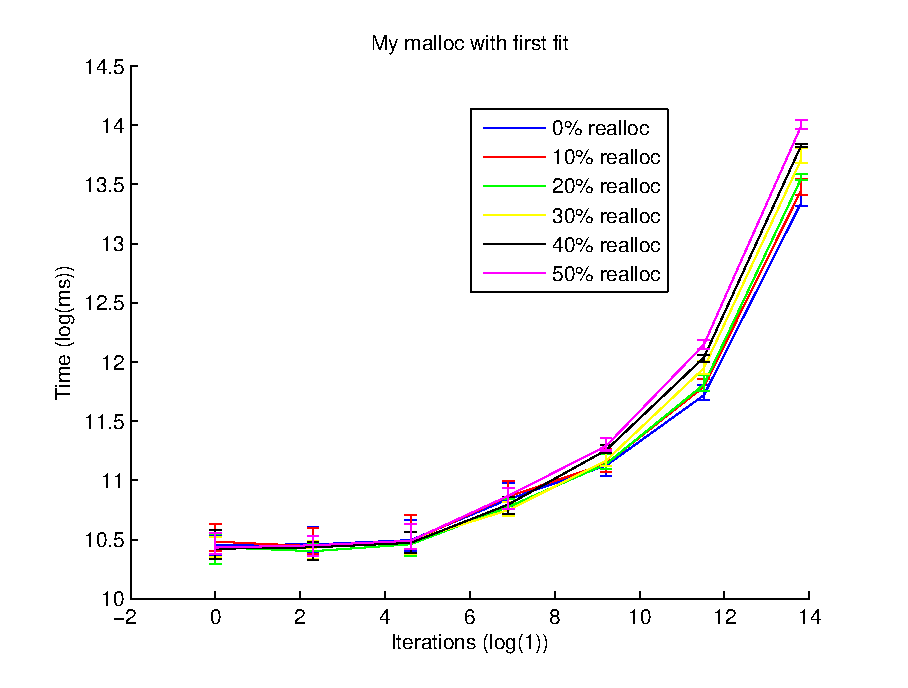
\includegraphics[scale=0.7]{../results/my1.eps}
\caption{Testkörning av min malloc() med first-fit och olika grader av realloc.}
\label{fig:digraph}
\end{figure}

\begin{figure}
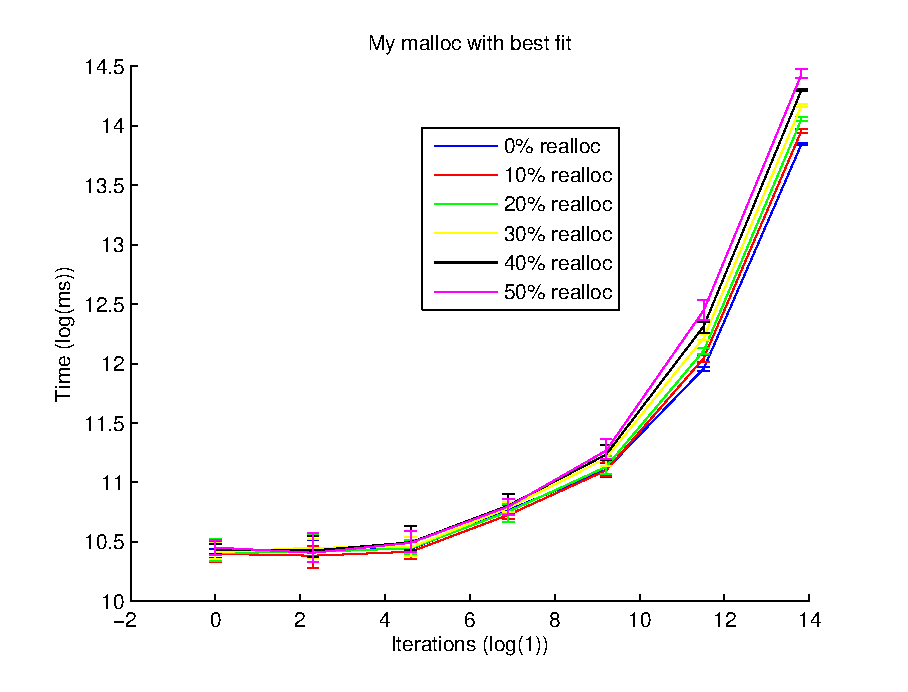
\includegraphics[scale=0.7]{../results/my2.eps}
\caption{Testkörning av min malloc() med best-fit och olika grader av realloc.}
\label{fig:digraph}
\end{figure}

\begin{figure}
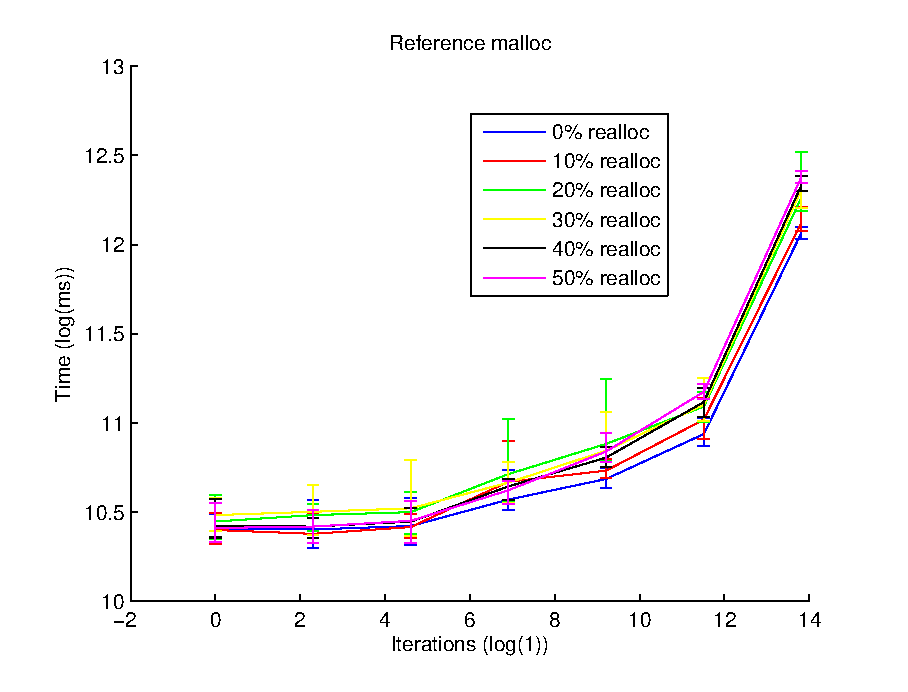
\includegraphics[scale=0.7]{../results/ref.eps}
\caption{Testkörning av systemets malloc() och olika grader av realloc.}
\label{fig:digraph}
\end{figure}

\begin{figure}
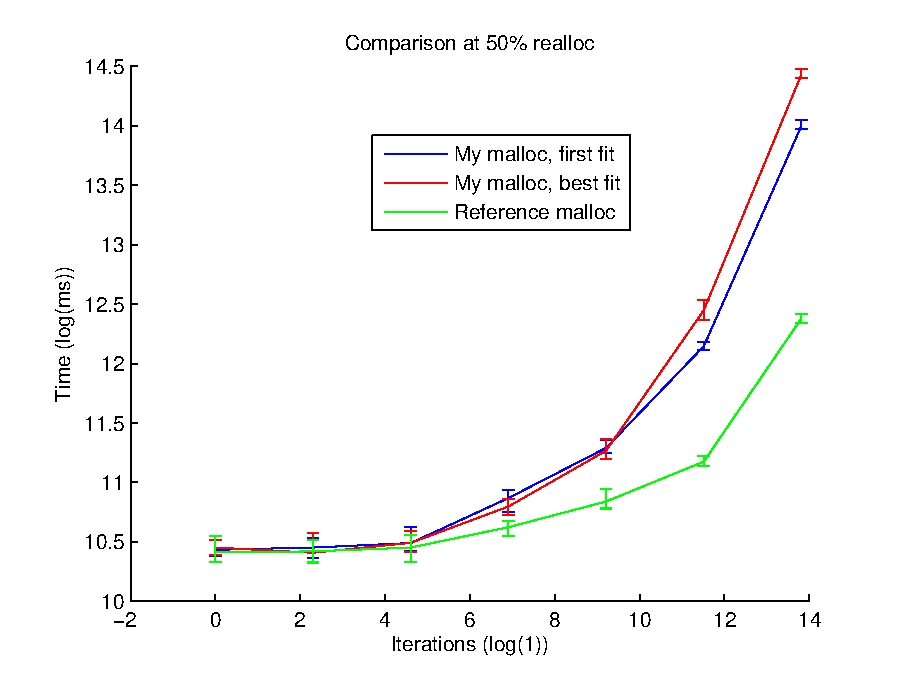
\includegraphics[scale=0.7]{../results/comparison.eps}
\caption{Jämförelse mellan de tre implementationerna vid 50\% realloc.}
\label{fig:digraph}
\end{figure}

\begin{lstlisting}

\end{lstlisting}


\clearpage
\section{Källkod}
Källkoden går att läsa nedan. Den går också att ladda ner från Github\footnote{\url{https://github.com/ZetaTwo/dd2200-laborationer/tree/master/labb3}} och kompileras med "make"

\subsection{malloc.c}
\lstinputlisting[style=cstyle]{../malloc.c}
\clearpage

\subsection{performancetest1.c}
\lstinputlisting[style=cstyle]{../performancetest1.c}
\clearpage

\section{Arbetsgång och Utvärdering}

TODO

\begin{itemize}
\item Labb-PM: X
\item Svårighetsgrad: X
\item Lärorikhet: X
\end{itemize}



\end{document}